\subsubsection{Time resolution}

As mentioned above six-bar method (see Sect.~\ref{sect:three-bar}) implies that six counters are put on top of each other. Since six-bar method demands multiple use of three-bar method different combinations of the counters are selected  as it shown on Fig.~\ref{6bar}. Then according to the formula~\ref{eq:resol_time} quantity $T$ for each bin from Fig.~\ref{fig:vert_cut} and for each selected three-bar combination is calculated using time-walk corrected times (see Sect.~\ref{sect:Time-walk}). $T$-distributions are plotted and fitted by gaussian. Since all counters are treated identically the formula~\ref{f:res}
can be written in this way:

\begin{equation}
\sigma_{avrg} = \sqrt{\frac{2}{3}}\sigma_T
\end{equation}
where $\sigma_T$ - spread of $T$-distributions and $\sigma_{avrg}$ -  resolution averaged over given three-bar combination.

On Fig.~\ref{fig:timeresol} the resolutions averaged over various three-bar combinations are plotted as function of the bar length. It can be noticed that resolution in the center of the bars is higher than at the edges. This happens because the combined time-walk effect has greater impact on the edges rather than in the middle. The average values of combined resolutions are shown on Fig.~\ref{fig:avrgtimeresol} for each three-bar combinations.
Then the same procedure is performed  for so-called complementary order. Permutations of the bars are shown on Fig.~\ref{6bar_compl}. .
Calculated values of average time resolution for normal and complimentary order of bar compinations are used as an input for system of linear equations~\ref{eq:linear_6bar} in order to extract individual resolutions of each counter as described in Sec.~\ref{sec:six-bars}.


\begin{figure}[]
\centering
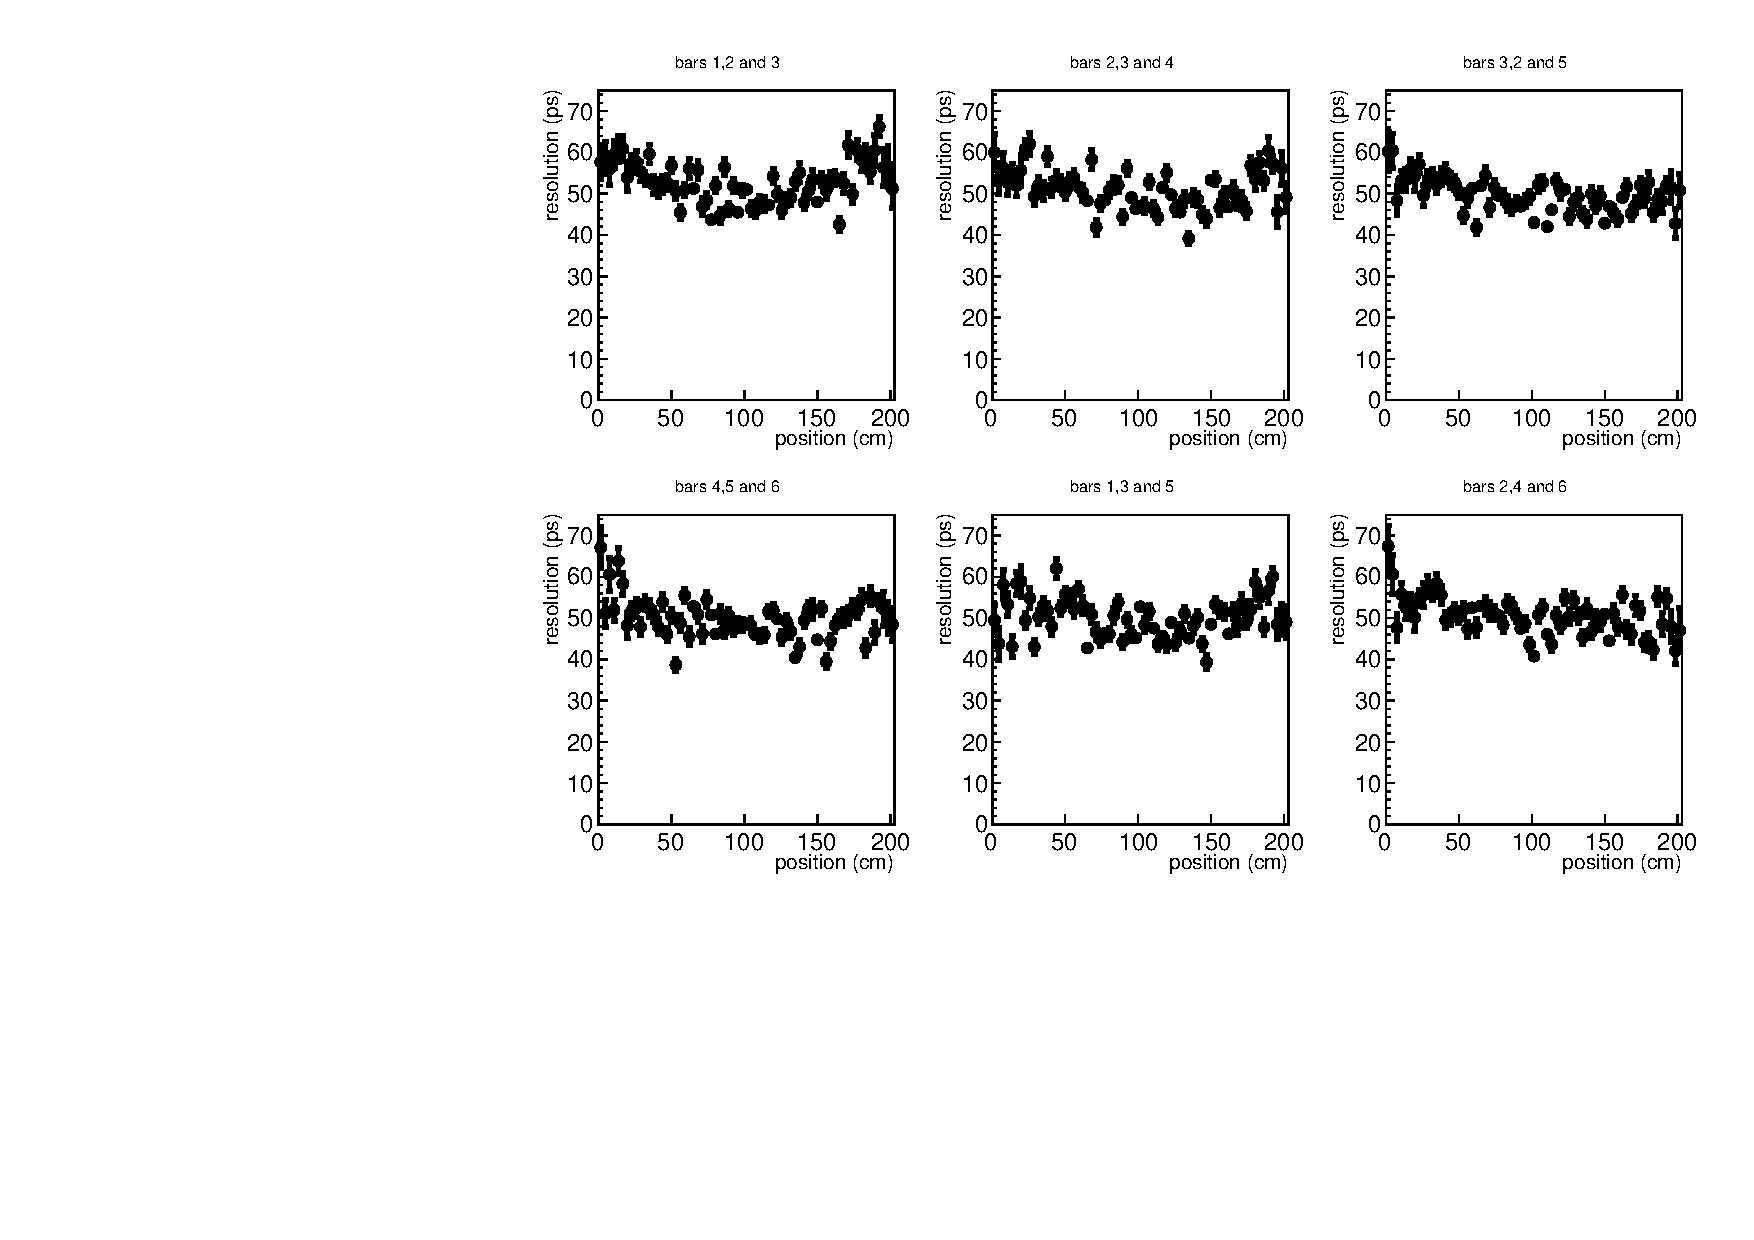
\includegraphics[width=0.6\textwidth]{gleb/fig_gleb_time_resol/resolution_203.pdf}
\caption{Time resolutions as function of position along the bar for 200 cm long bars from the set 30. Various plots represent various bars combinations\label{fig:timeresol}}
\end{figure}

\begin{figure}[]
\centering
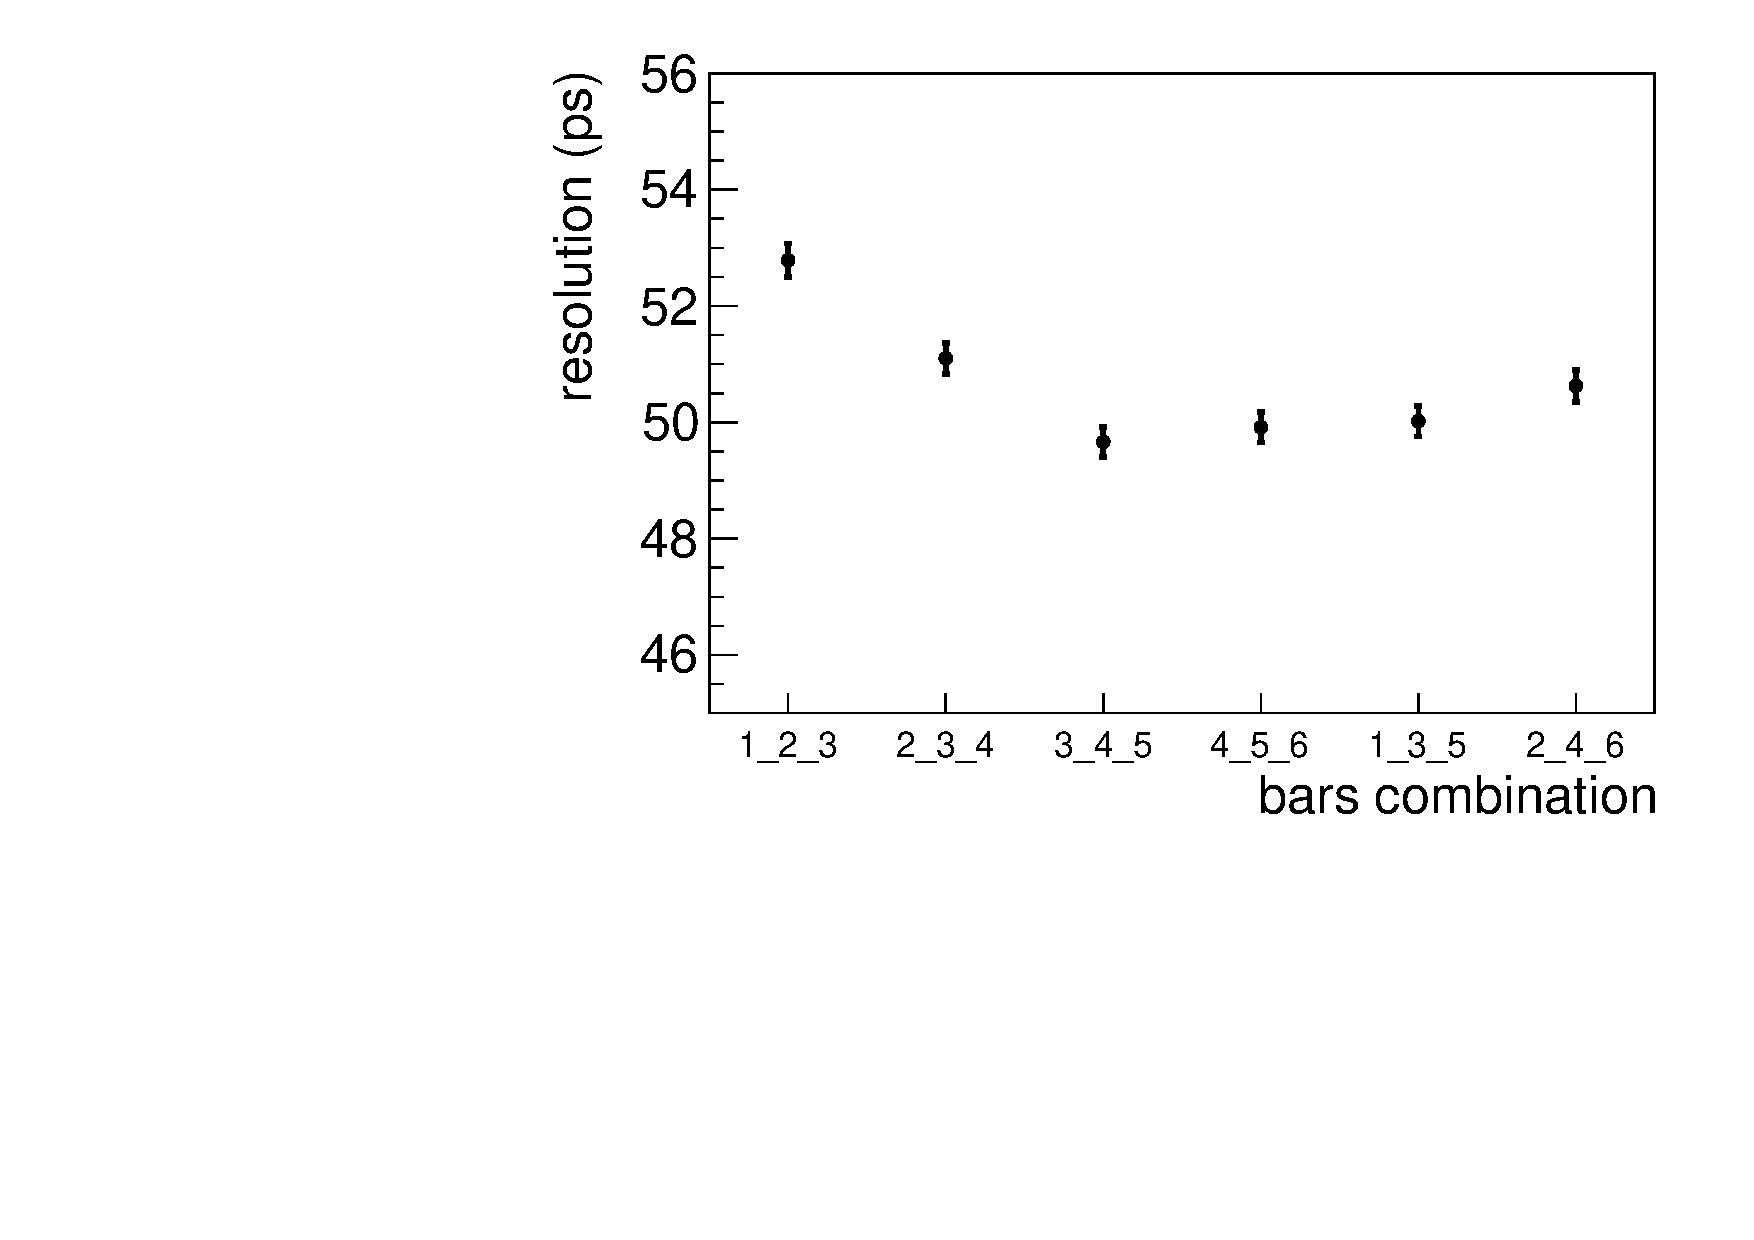
\includegraphics[width=0.6\textwidth]{gleb/fig_gleb_time_resol/avrg_resol_203.pdf}
\caption{Average time resolutions for various combinations of the bars. Plot corresponds to the 200 cm long bars from the set 30. \label{fig:avrgtimeresol}}
\end{figure}
